This Chapter summarises the structure of the information necessary 
to define the OpenQuake-engine PSHA input model. 
% -----------------------------------------------------------------------------
% -----------------------------------------------------------------------------
\section{Input Data definition}
Input data for probabilistic based seismic hazard analysis (Classical, 
Event based, Disaggregation, and UHS) are organised into:
\begin{itemize}
\item A general configuration file;
\item A file describing the Seismic Source System, that is the set of 
    initial source models and associated epistemic uncertainties needed 
    to model the seismic activity in the region of interest.
\item A file describing the Ground Motion System, that is the set of ground 
    motion prediction equations, per tectonic region type, needed to model 
    the ground motion shaking in the region of interest.
\end{itemize}

Figure \ref{fig:psha_input} summarises the structure of a PSHA input model
for the OpenQuake-engine and the relationships between the files.
% ..............................................................................
% . . . . . . . . . . . . . . . . . . . . . . . . . . . . . . . . . . . > Figure
\begin{figure}[!ht]
\centering
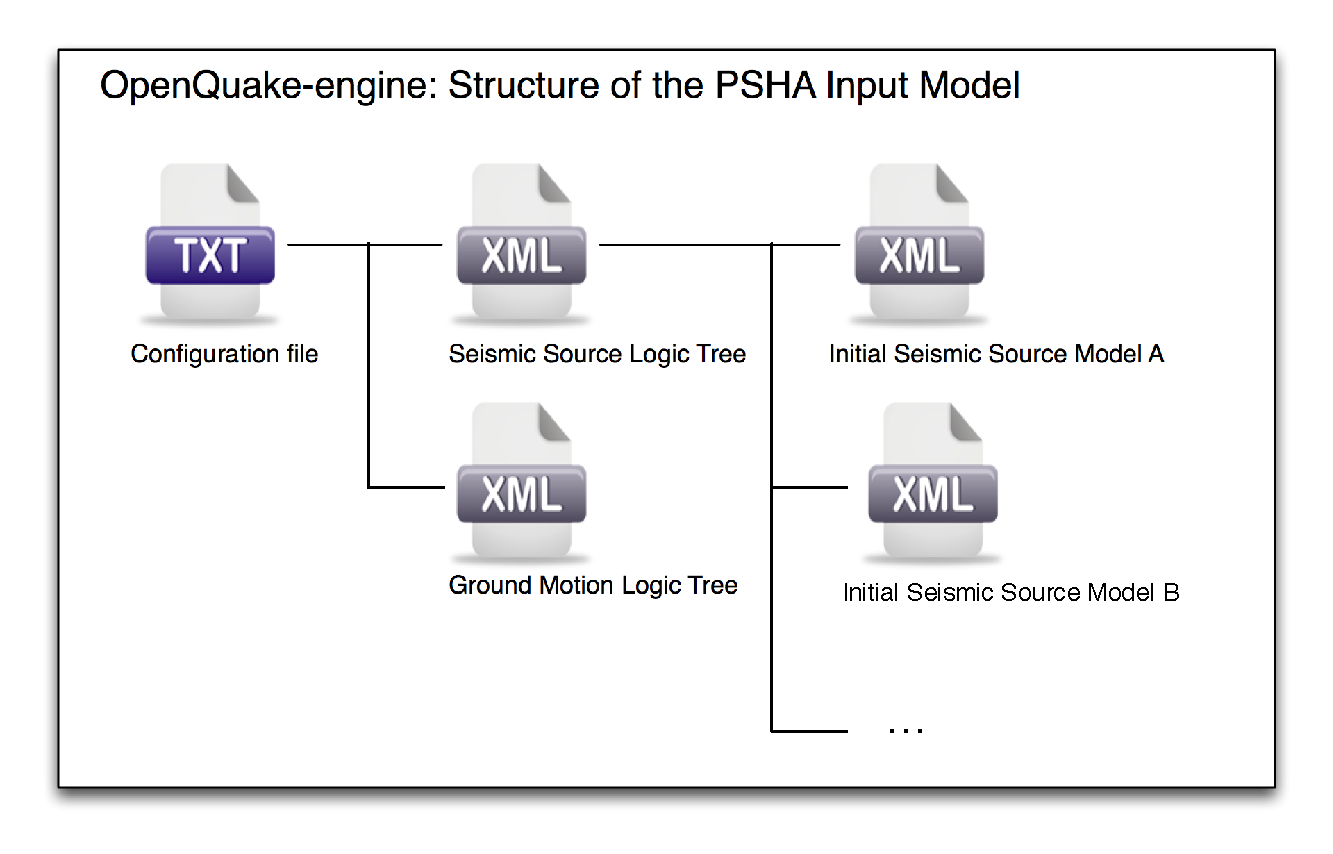
\includegraphics[width=14cm]{./figures/hazard/psha_input_structure.eps}
\caption{PSHA Input Model structure}
\label{fig:psha_input}
\end{figure}
% . . . . . . . . . . . . . . . . . . . . . . . . . . . . . . . . . . . < Figure
% ..............................................................................

% . . . . . . . . . . . . . . . . . . . . . . . . . . . . . . . . . . . . . . .
\subsection{The Seismic Source System}
The Seismic Source System contains the models describing position, geometry 
and activity of seismic sources of engineering importance for a set of sites
as well as the possible epistemic uncertainties to be incorporated into the 
calculation of seismic hazard.
%
% . . . . . . . . . . . . . . . . . . . . . . . . . . . . . . . . . . . . . . .
\subsubsection{The Seismic Source Logic Tree}
The structure of the Seismic Source Logic Tree consists of at least one 
branching level. The first - and mandatory - branching level is the one 
used to define one (or several) \glspl{initialseismicsourceinputmodel}
(see Figure \ref{fig:psha_input}). The successive branching levels can
be used to account for epistemic uncertainties in the parameters 
characterizing the \glspl{initialseismicsourceinputmodel}


The example provided below shows the simplest Seismic Source Logic Tree 
structure that can be defined in a PSHA Input model for OQ. This consists
of a logic tree with one initial seismic source model (with weight equal 
to one) and no epistemic uncertainties.
\input{./oqum/hazard/verbatim/sslt_example.tex}

The optional branching levels will contain rules that modify specific 
parameters of the sources in the initial seismic source model so as to 
take into account the epistemic uncertainties. 

For example, if the principal epistemic uncertainties to be considered are
source geometry and maximum magnitude, the modeller can create a logic tree
structure with three initial seismic source models (each one exploring a 
different definition of the geometry of sources and, an assigned weight) 
and one branching level accounting for the epistemic uncertainty on the 
maximum magnitude.
%
Below we provide an example of such logic tree structure.
\input{./oqum/hazard/verbatim/sslt_example_simpleLT.tex}
Note that the uncertainty on the maximum magnitude is specified in terms 
of relative increments with respect to the initial maximum magnitude 
defined in the initial seismic source models.
%
% . . . . . . . . . . . . . . . . . . . . . . . . . . . . . . . . . . . . . . .
\subsubsection{The Seismic Source Model}
\index{Input!Configuration file} 
The structure of the xml file representing the seismic source 
model corresponds to a list of sources, each one modelled using 
one out of typologies currently supported:
\input{./oqum/hazard/verbatim/ssm_sample.tex}
%
% . . . . . . . . . . . . . . . . . . . . . . . . . . . . . . . . . . . . . . .
\subsection{The Ground Motion System}
\index{Input!Ground motion system} 
The Ground Motion System defines the models and their possible epistemic 
uncertainties related to ground motion modelling to be incorporated 
into the calculation of seismic hazard.
%
% . . . . . . . . . . . . . . . . . . . . . . . . . . . . . . . . . . . . . . .
\subsubsection{The Ground Motion Logic Tree}
\index{Input!Ground motion logic tree} 
\label{ref:gmlt_example}
The structure of the \gls{groundmotionlogictree} consists of a list 
of ground motion prediction equations for each tectonic region used to
characterise the sources in the PSHA input model.

The example below shows a fairly simple \gls{groundmotionlogictree}. 
This Logic Tree assumes that all the sources in the PSHA input model 
belong to ``Active Shallow Crust'' and uses for calculation the 
\citet{chiou2008} \gls{acr:gmpe}.
\input{./oqum/hazard/verbatim/gmlt_example.tex}
%
% . . . . . . . . . . . . . . . . . . . . . . . . . . . . . . . . . . . . . . . 
% . . . . . . . . . . . . . . . . . . . . . . . . . . . . . . . . . . . . . . . 
\subsection{Configuration file}
\index{Input!Configuration file} 
\label{sec:conf_file}
The configuration file is the primary file controlling both the input 
model as well as parameters governing the calculation.

In this section we will illustrate different examples of the configuration
file addressing different typologies of seismic hazard calculation.
\subsubsection{Calculation of a hazard map and hazard curves using 
    the classical PSHA methodology}
\label{sec:config_classical_PSHA}
%
In the following we describe the overall structure and the
most typical parameters of a configuration file to be used for the 
computation of a seismic hazard map using a classical PSHA methodology.
\begin{itemize}
\item \textbf{Calculation type and model info}
\begin{Verbatim}[frame=single, commandchars=\\\{\}, fontsize=\small,
    numbers=left, numbersep=2pt]
[general]
description = A demo OpenQuake-engine .ini file for classical PSHA
calculation_mode = classical
random_seed = 1024
\end{Verbatim}
In this section the user specifies the following parameters:
\begin{itemize}
    \item \texttt{description}: a parameter that can be used to designate 
        the model 
    \item \texttt{calculation\_mode}: it is used to set the kind 
        of calculation. In this case it corresponds to \texttt{classical}.
        We'll describe alternative options later on.
    \item \texttt{random\_seed}: is used to control the random generator 
        so that when montecarlo procedures are used calculations are 
        replicable (if the same \texttt{random\_seed} is used you get 
        exactly the same results).
\end{itemize}
%
\item \textbf{Geometry of the area (or the sites) where hazard is computed}
    \hfill \\
This section is used to specify where hazard will be computed. Two 
option are available. 

The first one consists on defining a polygon 
(usually a rectangle) and a distance (in km) used to discretize the 
polygon area. The polygon is defined by a list of longitude-latitude tuples.

An example is provided below.
\begin{Verbatim}[frame=single, commandchars=\\\{\}, fontsize=\small,
    firstnumber=5, numbers=left, numbersep=2pt]
[geometry]
region = 10.0 43.0, 12.0 43.0, 12.0 46.0, 10.0 46.0
\# km
region_grid_spacing = 10.0
\end{Verbatim}

The second option allows the definition of a number of sites where 
the hazard will be computed. An example is provided below.
\begin{Verbatim}[frame=single, commandchars=\\\{\}, fontsize=\small,
    firstnumber=5, numbers=left, numbersep=2pt]
[geometry]
sites = 10.0 43.0, 12.0 43.0, 12.0 46.0, 10.0 46.0


\end{Verbatim}
If the list of sites is too long the user can specify the name 
of a .csv file as it is shown below
\begin{Verbatim}[frame=single, commandchars=\\\{\}, fontsize=\small,
    firstnumber=5, numbers=left, numbersep=2pt]
[geometry]
sites\_csv = <name_of_the_csv_file>


\end{Verbatim}
The format of the csv file containing the list of sites 
is a sequence of points (one per row) specified in terms 
of the longitude, latitude tuple. An example is provided below,
\begin{Verbatim}[frame=single, commandchars=\\\{\}, fontsize=\small,
    firstnumber=1, numbers=left, numbersep=2pt]
179.0,90.0
178.0,89.0
177.0,88.0
\end{Verbatim}


%
\item \textbf{Logic tree sampling} \hfill \\
    The \gls{acr:oqe} provides two options for processing the whole 
    logic tree structure. The first option uses Montecarlo sampling;
    the user in this case specifies a number of realizations. 

    In the second option all the possible realizations are created. 
    Below we provide an example for the latter option.
    In this case we set the \texttt{number\-\_of\-\_logic\_tree\_samples}
    to 0. \gls{acr:oqe} will perform a complete enumeration of all 
    the possible paths from the roots to the leaves of the logic tree 
    structure. 
\begin{Verbatim}[frame=single, commandchars=\\\{\}, fontsize=\small,
    firstnumber=9, numbers=left, numbersep=2pt]
[logic_tree]
number_of_logic_tree_samples = 0
\end{Verbatim}
    If the seismic source logic tree and the ground motion
    logic tree do not contain epistemic uncertainties the engine will
    create a single PSHA input.
%
\item \textbf{Parameters controlling the construction of the earthquake 
    rupture forecast}
\begin{Verbatim}[frame=single, commandchars=\\\{\}, fontsize=\small,
    firstnumber=11, numbers=left, numbersep=2pt]
[erf]
# km
rupture_mesh_spacing = 5
width_of_mfd_bin = 0.1
# km
area_source_discretization = 10
\end{Verbatim}
This section of the configuration file is used to specify the 
level of discretization of the mesh representing faults, the grid
used to delineate the area sources and, the magnitude-frequency 
distribution. 
Note that the smaller is the mesh spacing (or the bin width) the larger 
are (1) the precision in the calculation and (2) the computation demand.
%
\item \textbf{Parameters describing site conditions}
\begin{Verbatim}[frame=single, commandchars=\\\{\}, fontsize=\small,
    firstnumber=17, numbers=left, numbersep=2pt]
[site_params]
reference_vs30_type = measured
reference_vs30_value = 760.0
reference_depth_to_2pt5km_per_sec = 5.0
reference_depth_to_1pt0km_per_sec = 100.0
\end{Verbatim}
In this section the user specifies local soil conditions. The simplest
solution is to define uniform site conditions (i.e. all the sites have 
the same characteristics). Alternatively it's possible to define 
spatially variable soil properties in a separate file; the engine will
then assign to each investigation location the values of the closest point
used to specify site conditions.
%
\begin{Verbatim}[frame=single, commandchars=\\\{\}, fontsize=\small,
    firstnumber=17, numbers=left, numbersep=2pt]
[site_params]
site_model_file = ../_site_model/site_model.xml



\end{Verbatim}
The file containing the site model has the following 
structure:
\begin{Verbatim}[frame=single, commandchars=\\\{\}, fontsize=\small]
<?xml version="1.0" encoding="utf-8"?>
<nrml xmlns:gml="http://www.opengis.net/gml"
      xmlns="http://openquake.org/xmlns/nrml/0.4">
    <siteModel>
        <site lon="10.0" lat="40.0" vs30="800.0" 
            vs30Type="inferred" 
            z1pt0="19.367196734" z2pt5="0.588625072259" />
        <site lon="10.1" lat="40.0" vs30="800.0" 
            vs30Type="inferred" 
            z1pt0="19.367196734" z2pt5="0.588625072259" />
        <site lon="10.2" lat="40.0" vs30="800.0" 
            vs30Type="inferred" 
            z1pt0="19.367196734" z2pt5="0.588625072259" />
        <site lon="10.3" lat="40.0" vs30="800.0" 
            vs30Type="inferred" 
            z1pt0="19.367196734" z2pt5="0.588625072259" />
        <site lon="10.4" lat="40.0" vs30="800.0" 
            vs30Type="inferred" 
            z1pt0="19.367196734" z2pt5="0.588625072259" />
        ...
    </siteModel>
</nrml>
\end{Verbatim}

%
\item \textbf{Calculation configuration}
\phantomsection
\label{sec:calculation_configuration}
\begin{Verbatim}[frame=single, commandchars=\\\{\}, fontsize=\small,
     firstnumber=22, numbers=left, numbersep=2pt]
[calculation]
source_model_logic_tree_file = source_model_logic_tree.xml
gsim_logic_tree_file = gmpe_logic_tree.xml
# years
investigation_time = 50.0
intensity_measure_types = PGA, SA(0.1)
intensity_measure_types_and_levels = \{"PGA": [0.005, ..., 2.13]\} 
truncation_level = 3
# km
maximum_distance = 200.0
\end{Verbatim}
This section of the \gls{acr:oqe} configuration file specifies the 
parameters that
are relevant for the calculation of hazard. These include the names of
the two files containing the Seismic Source System and the Ground 
Motion System, the duration of the time window used to compute the 
hazard, the ground motion intensity measure types and levels for 
which the probability of exceedence will be computed, the level of
truncation of the gaussian 
distribution of the logarithm of ground motion used in the calculation 
of hazard and the maximum integration distance (i.e. the distance within 
which sources will contribute to the computation of the hazard).
%
\item \textbf{Output}
\begin{Verbatim}[frame=single, commandchars=\\\{\}, fontsize=\small,
    firstnumber=32, numbers=left, numbersep=2pt]
[output]
export_dir = out/
# given the specified `intensity_measure_types_and_levels`
quantile_hazard_curves =
poes_hazard_maps = 0.1
\end{Verbatim}
The final section of the configuration file is the one that contains 
the parameters controlling the typology of output to be produced.
%
\end{itemize}
%
%\input{config_file_event_based.tex}
%

\subsubsection{Seismic hazard disaggregation}
%
In this section we describe the structure of the configutation 
file to be used to complete a seismic hazard disaggregation. 
Since only a few parts of the standard configuration file need to 
be changed we'll use the description given in Section 
\ref{sec:config_classical_PSHA} at page 
\pageref{sec:config_classical_PSHA} as a reference and we'll 
emphasize herein major differences.
%
\begin{itemize}
%
\item \textbf{Calculation type and model info}
\begin{Verbatim}[frame=single, commandchars=\\\{\}, fontsize=\small]
[general]
description = A demo .ini file for PSHA disaggregation
calculation_mode = disaggregation
random_seed = 1024
\end{Verbatim}
The calculation mode parameter in this case is set as 
\texttt{disaggregation}.
%
\item \textbf{Geometry of the area (or the sites) where hazard is computed}
\begin{Verbatim}[frame=single, commandchars=\\\{\}, fontsize=\small]
[geometry]
sites = 11.0 44.5


\end{Verbatim}
In the section it will be necessary to specify the geographic 
coordinates of the site (or the sites) where the disaggregation
will be performed.
%
\item \textbf{Disaggregation parameters}
\begin{Verbatim}[frame=single, commandchars=\\\{\}, fontsize=\small]
[disaggregation]
poes_disagg = 0.02, 0.1
mag_bin_width = 1.0
distance_bin_width = 25.0
# decimal degrees
coordinate_bin_width = 1.5
num_epsilon_bins = 3
\end{Verbatim}
With the disaggregation settings shown above we'll disaggregate the intensity
measure levels with 10\% and 2\% probability of exceedance using the
\texttt{in\-ves\-ti\-gation\_time} and the intensity measure types 
defined in the ``Calculation configuration'' section of the OpenQuake
configuration file (see page \pageref{sec:calculation_configuration}). 

The parameters \texttt{mag\_bin\_width},  \texttt{distance\_bin\_width},
\texttt{coordinate\_bin\_width} control the level of discretization of the
disaggregation matrix computed. \texttt{num\_epsilon\_bins} indicates the 
number of bins used to represent the contributions provided by different
values of epsilon.

If the user is interested in a specific type of disaggregation,
we suggest to use a very coarse gridding for the parameters that are 
not necessary. For example, if the user is interested in a magnitude-distance 
disaggregation, we suggest the use of very large value for the 
\texttt{coordinate\_\-bin\_\-width} and to set  \texttt{num\_epsilon\_bins}
equal to 1.
\end{itemize}

\subsubsection{Event based PSHA}
%
In the following we describe the sections of the logic tree that are 
specific for event based PSHA calculations (the remaining sections 
\begin{enumerate}
\item \textbf{Calculation type and model info}
    This part is almost identical to the corresponding one 
    describe in section \ref{sec:config_classical_PSHA}. Note
    the setting of the \texttt{calculation\_mode} parameter.
\begin{Verbatim}[frame=single, commandchars=\\\{\}, fontsize=\small,
    numbers=left, numbersep=2pt]
[general]
description = A demo OpenQuake-engine .ini file for classical PSHA
calculation_mode = event_based
random_seed = 1024
\end{Verbatim}
%
\item \textbf{Event based} \hfill \\
This is an additional part used to specify the number of stochastic 
event sets (each one representing a potential realisation of seismicity
during the \texttt{investigation\_time} specified in the 
\texttt{calculation\_configuration} part.
\begin{Verbatim}[frame=single, commandchars=\\\{\}, fontsize=\small]
[event_based_params]
ses_per_logic_tree_path = 5
ground_motion_correlation_model = JB2009
ground_motion_correlation_params = {"vs30_clustering": true}
\end{Verbatim}
%
\item \textbf{Output} \hfill \\
This part substitutes the \texttt{Output} part described in 
configuration file example descibed in section \ref{sec:config_classical_PSHA}
at page \pageref{sec:config_classical_PSHA}.
\begin{Verbatim}[frame=single, commandchars=\\\{\}, fontsize=\small]
[output]
export_dir = /tmp/xxx
complete_logic_tree_ses = true
complete_logic_tree_gmf = true
ground_motion_fields = true
# post-process ground motion fields into hazard curves,
# given the specified `intensity_measure_types_and_levels`
hazard_curves_from_gmfs = true
mean_hazard_curves = true
quantile_hazard_curves = 0.15, 0.5, 0.85
poes_hazard_maps = 0.1, 0.2
\end{Verbatim}
%
\end{enumerate}

